\documentclass{article}
\usepackage{tikz}
\begin{document}
  \begin{center}
    \begin{figure}
      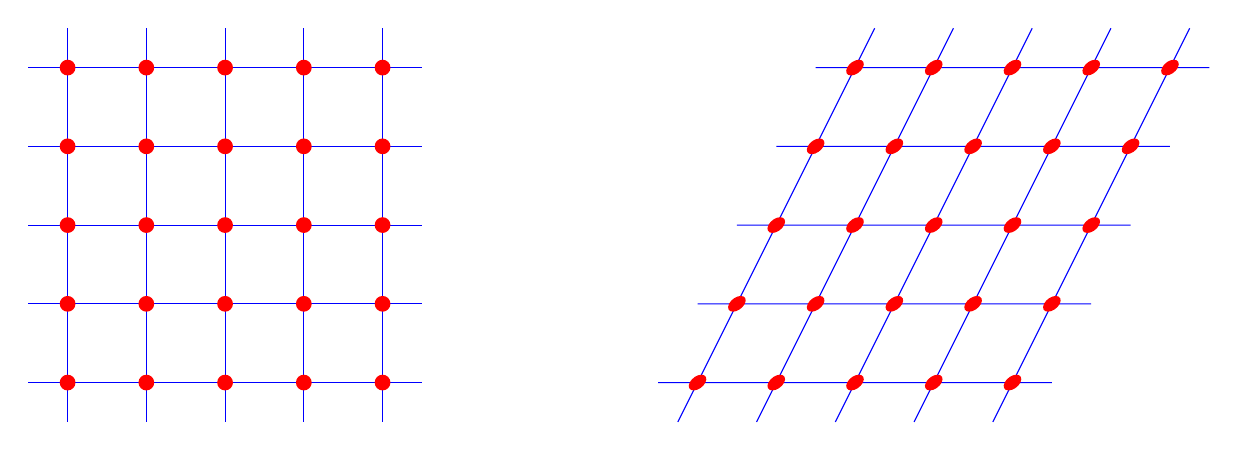
\begin{tikzpicture}[scale=0.5]
        \draw[step=2cm, thin, blue] (-5,-5) grid (5,5);
          \foreach \x in{-4,-2,0,2,4}
          {
              \foreach \y in{-4,-2,0,2,4}
              {
                \fill[red] (\x,\y) circle [radius =0.2];
              }
          }
          
        \begin{scope}[xshift=18cm, xslant=0.5]
            \draw[step=2cm, thin, blue] (-5,-5) grid (5,5);
              \foreach \x in {-4,-2,0,2,4}
              {
                \foreach \y in {-4,-2,0,2,4}
                {
                    \fill[red] (\x,\y) circle [radius=0.2];
                }
            }
        \end{scope}
    \end{tikzpicture}
    \label{lattice}
    \caption{Lattice}
    \end{figure}
\end{center}
\end{document}
